\input{settings}
\setlength{\emergencystretch}{2em}
\titleformat{\section}
  {\small\bfseries\raggedright}
  {}{0em}
  {}
  [{\color{WHU_Blue}\titlerule}]
\titlespacing*{\section}{0cm}{0.75em}{0.52em}
\titlespacing*{\subsection}{0cm}{0.50em}{0.30em}
\setlist[itemize]{topsep=0.15em, itemsep=0.15em, parsep=0em, partopsep=0em, leftmargin=1.25em}
\setlist[enumerate]{topsep=0.15em, itemsep=0.15em, parsep=0em, partopsep=0em, leftmargin=1.35em}
\renewcommand{\arraystretch}{0.98}
\renewcommand{\CJKglue}{\hskip 0.018em}

% 个人信息
% cd template && xelatex -interaction=nonstopmode main_guoqi.tex && xelatex -interaction=nonstopmode main_guoqi.tex
\newcommand{\school}{江南大学 · 控制科学与工程}

\newcommand{\resumeDecor}{
    \begin{tikzpicture}[remember picture, overlay]
        \node[anchor=north, inner sep=0pt](header) at (current page.north){
            
\includegraphics[width=\paperwidth]{images/header.png}
        };
        \node[anchor=west](school_logo) at (header.west){
            \hspace{0.5cm}
            
\includegraphics[width=0.15\textwidth]{images/whu_logo_1.png}
        };
        \node[anchor=east](school_name) at(header.east){
            \textcolor{white}{\textbf{\school}}
            \hspace{0.5cm}
        };
    \end{tikzpicture}

    \begin{tikzpicture}[remember picture, overlay]
        \node[opacity=0.05] at(current page.center){
            
\includegraphics[width=0.68\paperwidth, keepaspectratio]{images/whu_logo_big.png}
        };
    \end{tikzpicture}
}

\newcommand{\sectionIcon}[2]{\makebox[\widthof{#1}][c]{\color{WHU_Blue}{#1}}\quad #2}

%%%%%%%%%%%%%%%%%%%%
% 简历正文（国企/央企导向：政治面貌与校园组织经历前置）
%%%%%%%%%%%%%%%%%%%%
\begin{document}
\resumeDecor
\vspace*{-3.15em}
\scriptsize
\linespread{1.08}\selectfont

% 个人信息
\begin{minipage}{0.80\textwidth}
    \section[个人信息]{\sectionIcon{\faAddressCard}{个人信息}}
    \footnotesize
    \begin{tabularx}{\linewidth}{p{\widthof{求职意向:}}Xp{\widthof{最高学历:}}X}
        姓\ \ \ \ \ \ \ \ 名: & 梁邦一 &
        性\ \ \ \ \ \ \ \ 别: & 男 \\
        政治面貌: & \hl{中共党员} &
        电\ \ \ \ \ \ \ \ 话: & +86 15515602693 \\
        邮\ \ \ \ \ \ \ \ 箱: & yuejinai55@gmail.com &
        求职意向: & 研发 / 工程技术类 \\
    \end{tabularx}
\end{minipage}
\hfill
\begin{minipage}{0.11\textwidth}
    \vspace{2.0em}
    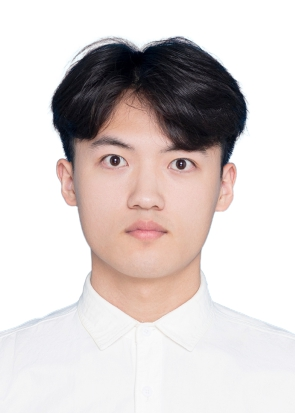
\includegraphics[width=\linewidth]{images/avatar.png}
\end{minipage}
\vspace{-0.60em}

\section[教育背景]{\sectionIcon{\faGraduationCap}{教育背景}}
\begin{itemize}
    \item {\textbf{控制科学与工程硕士，江南大学}}（\hl{中国科学院沈阳自动化研究所 · 机器人与智能系统全国重点实验室联合培养}） \hfill {2024.06--2027.06}
    \item {\textbf{自动化学士，郑州轻工业大学}}（自动化原理、传感器与检测、微机原理、嵌入式系统） \hfill {2020.09--2024.06}
\end{itemize}

% 校园与组织经历
\section[校园与组织经历]{\sectionIcon{\faUsers}{校园与组织经历}}
{\small\textbf{硕士党支部书记}}\quad 江南大学控制科学与工程硕士支部 \hfill {2024.10--2026.05} \\
{\scriptsize\color{WHU_Blue} 支部建设 / 组织生活 / 成员协调}
\begin{itemize}
    \item 组织支部活动与成员协调，保障支部事务稳妥推进。
    \item 与本科学段班长经历合计 \hl{6 年学生干部经历}，沉淀跨角色沟通、需求收集、任务拆解与落地推进能力。
\end{itemize}

\vspace{0.30em}
{\small\textbf{本科班长}}\quad 郑州轻工业大学自动化专业 \hfill {2020.10--2024.06} \\
{\scriptsize\color{WHU_Blue} 班级统筹 / 活动组织 / 师生桥梁}
\begin{itemize}
    \item 统筹管理 \hl{60 人班级}事务：对接学院老师传达教学任务与活动安排，组织班级分工合作，收集并解决同学在学业与生活中的共性问题。
    \item 策划 \hl{3 场以上大型班级活动}，持续提升班级凝聚力，确保教学任务与活动安排信息通畅。
\end{itemize}

% 荣誉奖项
\section[荣誉奖项]{\sectionIcon{\faStar}{荣誉奖项}}
\begin{itemize}
    \item 中国机器人大赛暨 RoboCup 机器人世界杯中国赛 \hl{国家三等奖}；校一等奖学金（2025.10、2026）；\hl{优秀毕业生}（2024.06）；\hl{优秀班干部}（2022.10）。
\end{itemize}

% 专业技能
\section[专业技能]{\sectionIcon{\faWrench}{专业技能}}
\begin{itemize}
    \item \textbf{工程落地与执行}：Python、C++、Linux / Ubuntu、Git、PLC 编程、控制逻辑设计、设备规格书解读、流程图与方案文档。
    \item \textbf{AI 与数据}：PyTorch、Ultralytics YOLO、Qwen3-VL、LLaMA-Factory、TensorRT、ONNX、NVIDIA Jetson AGX Orin、H20 8GPU 分布式训练。
    \item \textbf{数据工程}：多源数据清洗、标注质检、训练/验证/测试集划分、标签库建设。
    \item \textbf{协同与文档}：需求转技术方案、方案评审、Markdown / LaTeX 结构化文档、运行记录与交接文档、Claude Code / Codex AI 工作流。
\end{itemize}

% 实习经历
\section[实习经历]{\sectionIcon{\faBriefcase}{实习经历}}
{\small\textbf{CARIZON（大众×地平线合资智驾）}}\quad 感知数据部门算法实习生 \hfill {2026.06--至今}\\
{\scriptsize\color{WHU_Blue} 数据挖掘 / 大模型后训练 / 业务交付}
\begin{itemize}
    \item 融合车载多路传感器与回灌数据设计规则化挖掘算子，红绿灯自车转向 Tagger 在 3W 条路口数据中筛选 3K 条 CLIP，\hl{验收 90\%、挖掘召回提升 10\%}。
    \item 负责感知细粒度识别 VLM 后训练优化：围绕闸机杆五分类完成数据清洗、标注校验与 Prompt 迭代，基于 Qwen3-VL-8B + LLaMA-Factory 在 H20 8GPU 集群完成全参数 SFT，\hl{测试集准确率 0.8984 创历史新高}。
\end{itemize}

\vspace{0.30em}
{\small\textbf{优奇智能科技有限公司（优必选子公司）}}\quad 人形机器人感知算法实习生 \hfill {2026.02--2026.05} \\
{\scriptsize\color{WHU_Blue} 模型训练复现 / 数据质检 / bad case 归因}
\begin{itemize}
    \item 负责 R11 接待机器人感知模型在 NVIDIA Jetson AGX Orin 端侧计算平台的部署，围绕 TensorRT 完成 PyTorch $\rightarrow$ ONNX $\rightarrow$ TensorRT 模型转换、量化与算子优化，\hl{推理延迟降低 20\%}，在真机跑通检测/分割实时推理链路。
    \item 参与 R11 接待机器人 YOLO11s-seg 模型训练复现与多场景数据质检、训练/验证/测试划分，\hl{推动检测/分割训练链路跑通}；围绕误检漏检 bad case 归因，\hl{将模型效果问题转化为可执行的数据侧优化需求}。
\end{itemize}

\vspace{0.30em}
{\small\textbf{长兴和良智能制造有限公司}}\quad 研发实习生 \hfill {2024.05--2024.09} \\
{\scriptsize\color{WHU_Blue} 制造业一线 / PLC 控制程序优化 / 生产验证}
\begin{itemize}
    \item 负责汽车空调弯管机 \textbf{PLC 控制程序优化项目}：独立完成设备规格书解读、控制逻辑设计与流程文档输出，\hl{优化方案在实际生产环境稳定运行}，积累"现场需求 → 控制逻辑 → 交付验证"完整工程经验。
\end{itemize}

% 科研与项目经历
\section[科研与项目经历]{\sectionIcon{\faFlask}{科研与项目经历}}
{\small\textbf{面向具身智能灵巧操作的肌电-力融合感知与灵巧手抓取控制系统（灵心巧手） · 负责人}} \hfill {2025.02--2026.02} \\
{\scriptsize\color{WHU_Blue} 端到端项目负责人 / 多传感器融合 / 团队协同}
\begin{itemize}
    \item \textbf{独立牵头}多模态感知系统从 0 到 1 建设，拆解为硬件采集 → 算法训练 → 仿真验证 → ROS2 联调 → 演示交付 5 大阶段，\hl{历时 12 个月完成端到端项目闭环}；统筹设备、算力与人员节奏，保障各阶段按期启动。
    \item 在机器人与智能系统全国重点实验室（中国科学院沈阳自动化研究所）承担课题实验链路组织与训练环境保障，独立完成 \hl{Linux 服务器环境搭建与维护}；系统梳理方向英文文献，\hl{支撑 IEEE Sensors Journal 综述写作}。
\end{itemize}

% 论文与研究成果
\section[论文与研究成果]{\sectionIcon{\faBook}{论文与研究成果}}
\begin{itemize}
    \item \hl{已录用 · 第一作者}（JCR 一区 / 中科院二区）：Liang B., Li N., Li G., et al. Sensing Technologies for Hand Gesture Recognition in Human-Robot Interaction: A Review[J]. IEEE Sensors Journal, 2025, 26(2): 1501-1519. \textbf{综述}：梳理数据手套、视觉与肌电等手势感知路线，对比精度、侵入性与成本取舍。
    \item \hl{In Revision（在修）}（JCR 一区 / 中科院二区 Top）：sEMG Conformer: Synergizing Local-Global Spatiotemporal Features for Continuous Force Estimation. Biomedical Signal Processing and Control. \textbf{算法核心}：卷积局部感受野 + 自注意力全局建模，解码肌电—指尖力映射，单模型支持力等级分类与连续力值回归。
    \item \hl{Under Review（在投）}（JCR 一区 / 中科院二区）：Dexterous Hand Grasping Control Based on Multimodal Sensory Fusion and Simulation Reinforcement Learning. \textbf{系统闭环}：MuJoCo 仿真强化生成抓取姿态，融合视觉、肌电与触觉构建分层控制链路，G20 上完成闭环部署验证。
\end{itemize}

\end{document}
